% makale_orbit_bastirma.tex — English paper draft (REVTeX 4.2, PRAB style)
% Kaynak taslak: makale_orbit_bastirma.md (Türkçe iskelet + düz metin)
% Figürler: make_orbit_figures.py (fig_orbit_*.png); C++ verisi kmod_drivers/paper_runs.py
%
% ============================================================================
% YENİDEN YAZIM (2026-07): jargon azaltıldı (aşina olmayan okur için düz dil),
% null-BBA iterasyonu TAMAMLANMIŞ C++ sonucuyla güncellendi (356×→145×; dikey
% çözülüyor, yatay takılıyor), ve yatay-düzlem tıkanmasının dürüst nedeni
% düzeltildi: "dispersiyon" değil — analitik yönlendirme modeli deflektörleri
% DRIFT sayıyor (yatay odaklama + dispersiyon modelde yok); dikeyde deflektör
% ~odaklamıyor, o yüzden dikey model doğru ve BBA çalışıyor. Kaynak:
% separation_bba_testleri.md §5.2, analytic_kmod.py compute_twiss_at_quads.
% AŞIRI-İDDİADAN KAÇIN: null-BBA tam çözüm değil (yatay + donanım tabanı açık).
% ============================================================================
\documentclass[aps,prab,reprint,superscriptaddress,nofootinbib]{revtex4-2}

\usepackage{graphicx}
\usepackage{amsmath,amssymb}
\usepackage{bm}
\usepackage[colorlinks=true,linkcolor=blue,citecolor=blue,urlcolor=blue]{hyperref}

\begin{document}

\title{Suppression of the quadrupole-misalignment false EDM signal by
orbit-based methods in a proton EDM storage ring, and its limits}

\author{S. Hac{\i}\"omero\u{g}lu}
\affiliation{Affiliation}

\date{\today}

\begin{abstract}
The proposed storage-ring experiment for the proton electric dipole moment
(EDM) must detect a spin rotation of about one nanoradian per second.  At that
level, quadrupole magnets displaced from their ideal positions by only a few
microns produce a spin signal that imitates a real EDM.  This ``false EDM''
comes from a geometric (Berry) phase and grows as the \emph{square} of the
misalignment, so at a realistic alignment of $10~\mu$m it is about a thousand
times larger than the target.  We ask a simple question with a simulation of
the ring: how much of this false signal can be removed by measuring and
correcting the beam orbit, the everyday toolbox of accelerator alignment?
Standard orbit correction, together with running clockwise and
counter-clockwise beams at once, removes a factor of about $26$, but no
further.  The reason is that the leftover misalignment lives in a special
pattern --- neighboring quadrupoles displaced \emph{together} --- whose effect
on the orbit is roughly a hundred times weaker than for the opposite pattern.
We show that a whole family of orbit techniques (matrix inversion, per-magnet
gradient modulation read as an amplitude, neural networks, drift monitoring,
harmonic fits, and the counter-rotating beam separation) all stall at the same
floor, and that the floor is set not by detector noise --- which can be
averaged away --- but by two coherent effects that cannot: the optics
``breathing'' when a magnet is modulated, and the mismatch between the real
optics and the model used to analyze it.  Better beam-position monitors,
including SQUID-based ones, do not move this floor.  We then identify one
technique that escapes it: null-finding beam-based alignment (BBA), which
locates each magnet center by the beam position where the orbit stops
responding.  A zero-crossing does not care about the response size, so it is
not blocked by these walls.  In idealized optics it recovers the hidden
pattern and cuts the false EDM from $356\times$ to $1.6\times$ target.  Under
realistic optics errors it works in the vertical plane after the orbit is first
flattened and the procedure iterated.  The horizontal plane at first stalled;
we traced this to the steering model, which treats the electric deflectors as
field-free drifts --- accurate vertically but not in the bending plane --- and
showed that steering with the ring's measured response matrix instead corrects
the horizontal magnets and lowers the false-EDM floor about nine-fold, to
$\sim\!17\times$ target.  We present this as the one promising route, its main
obstacle understood and demonstrably fixed but not yet a finished solution (the
horizontal plane still trails the vertical and a hardware floor remains), and
conclude that reaching the target by the other techniques would require the
symmetric misalignment to be held below about $1~\mu$m by construction, a
tolerance that no orbit measurement can verify.
\end{abstract}

\maketitle

% ═══════════════════════════════════════════════════════════════════
\section{Introduction}
\label{sec:intro}

\subsection{The experiment: searching for a proton EDM}

An electric dipole moment (EDM) is a tiny separation of a particle's positive
and negative charge along its spin.  If it exists, it breaks time-reversal
symmetry, and finding one in the proton above the Standard-Model level
($\lesssim 10^{-31}\,e\!\cdot\!$cm) would be direct evidence of new physics.
The proposed storage-ring experiment~\cite{omarov} aims for
$d = 10^{-29}\,e\!\cdot\!$cm.

The method is called \emph{frozen spin}.  Protons circulate at a special
``magic'' momentum ($p \approx 0.7$~GeV/$c$) in a ring that bends the beam with
electric fields and focuses it with magnetic quadrupoles.  At this momentum the
spin stays pointed along the direction of motion; it does not drift ahead or
behind within the ring plane.  If the proton has an EDM, the ring's radial
electric field slowly tips the spin \emph{out} of that plane.  The measured
quantity is the rate of that tip,
\begin{equation}
  f \equiv \frac{dS_y}{dt}, \qquad
  d = 10^{-29}\,e\!\cdot\!\text{cm} \;\leftrightarrow\;
  f \approx 1~\text{nrad/s} ,
  \label{eq:target}
\end{equation}
one radian in about thirty years.  Every other effect that can tip the spin
out of plane at this level must be removed or safely bounded.  Effects that
imitate the EDM are called \emph{false EDM} signals; this paper is about the
most stubborn one.

\subsection{The false EDM: a geometric phase from misalignments}

The ring has 48 quadrupole magnets, and in practice each sits a few microns
away from its ideal place.  A quadrupole has zero field at its center, so a
beam passing off-center feels a field proportional to how far off it is.  Which
way the magnet is displaced decides what it does to the spin.  A \emph{vertical}
offset $dy$ gives the beam a radial field that rotates the spin about the
horizontal ($x$) axis.  A \emph{horizontal} offset $dx$ gives it a vertical
field that rotates the spin about the vertical ($y$) axis.

Either rotation on its own is nearly harmless, because it averages out around
the ring.  Trouble comes when both are present at once.  Rotations about
different axes \emph{do not commute}: rotating first about $x$ and then about
$y$ is not the same as doing them in the other order, and the small leftover
difference builds up turn after turn into a net rotation about the third axis
--- exactly the out-of-plane direction where the EDM is sought.  This is the
familiar geometric (Berry) phase.  Its size is
\begin{equation}
  f_{\text{false}} \;\propto\; dx \cdot dy
  \;\;\Longrightarrow\;\;
  f_{\text{false}} \propto \sigma^2 ,
  \label{eq:sigma2}
\end{equation}
so it depends on the \emph{product} of the two offsets, and therefore grows as
the \emph{square} of the rms misalignment $\sigma$.  We verify the square law
directly in Sec.~\ref{sec:estimator} (measured exponent $p = 2.00 \pm 0.01$,
matching Fig.~9(a) of Ref.~\cite{omarov}).  The number is unforgiving: at
$\sigma = 10~\mu$m the false EDM is about $1000\times$ the target, and it lives
in the \emph{same} measured quantity, $dS_y/dt$, as the real signal.

The obvious hope is that the beam itself can be used as the ruler.  The ring's
48 beam-position monitors (BPMs) continuously read where the beam sits;
misaligned quadrupoles bend that path; so measuring the misalignments from the
orbit and correcting them --- the standard \emph{beam-based alignment} (BBA)
practice --- ought to clean up the false EDM as well.  This paper measures how
far that hope holds, and where and why it stops.

\subsection{What is already known}

Most pieces of this problem are, individually, solved.  Our contribution is to
put them together around the false-EDM question.

\paragraph{Orbit correction and observability.}
Correcting the orbit by singular-value decomposition (SVD) of the response
matrix --- including the idea of poorly-visible modes and how to reject them
--- goes back to Chung, Decker, and Evans~\cite{chung1993}.  The gain law we
use throughout, $G_k = C/|Q^2-k^2|$, is the harmonic limit of that picture.
The bias of estimators when the orbit-response inversion is nearly degenerate
was worked out by Wegscheider and Vilsmeier~\cite{wegscheider}; their
degenerate parameter is the quadrupole strength, ours the transverse offset.

\paragraph{Beam-based alignment.}
Steering the beam through quadrupole centers is routine: vary a quadrupole's
strength and find the beam position where the orbit stops responding, speed it
up with ac excitation~\cite{marti}, and do many magnets at once~\cite{huang}.
None of the measurement techniques we test is new.  \emph{What is new is
measuring how well each one does on the specific misalignment pattern that
drives the false EDM.}

\paragraph{False-EDM budgets.}
The forward calculation, misalignment~$\to$~false EDM, was done for an
all-electric ring in Ref.~\cite{haciomeroglu2017}.  The full systematic budget
of the magnetic-quadrupole symmetric-hybrid design is given by Omarov \emph{et
al.}~\cite{omarov}, who show the geometric-phase false EDM can be brought below
target by combining clockwise (CW) and counter-clockwise (CCW) beams,
quadrupole polarity switching, and shrinking the separation between the two
counter-rotating (CR) beams with dipole correctors.

\paragraph{Neighboring work.}
Orbit correction in symmetric lattices~\cite{mirza}; updating the response
matrix on line~\cite{ziemann}; the orbit imprint of ground motion~\cite{rossbach};
polarimeter performance and statistics~\cite{polarimeter}.

\subsection{The open gap}

The control chain of Ref.~\cite{omarov} relies on \emph{measuring} the CR beam
separation and reducing it.  Three things are left open there.  (i) The
measurement chain itself --- 48 BPMs (or SQUID pickups) plus the reconstruction
--- is not simulated.  (ii) A possible blindness to the part of the
misalignment that the orbit cannot see is not addressed.  (iii) Whether
polarity switching is a separate handle from CW/CCW reversal is not quantified.
These matter because, as we show, the part of the misalignment that drives the
residual false EDM is exactly the part the orbit sees least.

\subsection{This paper}

With realistic BPM systematics (offsets, gain errors, noise) and optics-model
errors ($\beta$-beating, quadrupole tilt), we find the false-EDM floor
reachable by orbit measurement and correction, as a function of the alignment
tolerance.  At $\sigma = 10~\mu$m the floor is
$\sim\!6\times10^{-28}\,e\!\cdot\!$cm, and it scales as $\sigma^2$.  We show the
floor is \emph{independent of BPM technology}: it is set not by random noise but
by two coherent effects that do not average down.  And we identify one
technique --- null-finding BBA --- that is not subject to these walls, map how
far it currently reaches, and state honestly where it stalls.

Section~\ref{sec:method} describes the simulation, the false-EDM estimator, the
symmetric/antisymmetric split, and the error models.
Section~\ref{sec:results} first establishes the suppression that orbit control
does deliver, then walks through each attempt to recover the hidden component
and where it stops, and finally presents null-finding BBA.
Section~\ref{sec:conclusions} draws the conclusions for the experiment.

% ═══════════════════════════════════════════════════════════════════
\section{Method}
\label{sec:method}

\subsection{Two simulation tools}

Every number here comes from one of two tools that share only the configuration
file, so agreement between them cannot come from a shared modeling mistake.

\paragraph{Full particle-and-spin tracker (C++).}
The ring --- electric bending sections plus 24 FODO cells with 48 magnetic
quadrupoles ($R_0 = 95.49$~m, $g \approx 0.2$~T/m, vertical tune
$Q_y \approx 2.3$) --- is pushed through the real fields element by element with
a fourth-order Gauss--Legendre \emph{symplectic} integrator, and the spin rides
along in the same steps via the Thomas-BMT equation.  ``Symplectic'' means the
integrator does not let energy or amplitude errors creep up over long tracking,
which is what makes a nrad/s slope measurable at all.  The real EDM enters
through a switch
($\eta = 1.88\times10^{-15} \rightarrow dS_y/dt = 9.81\times10^{-10}$~rad/s,
odd under CW/CCW, matching Eq.~(C1) of Ref.~\cite{omarov}).  All false-EDM runs
have the EDM switch \emph{off}, so any vertical spin rotation we see is, by
construction, a systematic.

\paragraph{Analytic Twiss / closed-orbit solver.}
From the $2\times2$ transfer matrices of the quadrupoles and drifts we build the
lattice functions $\beta(s)$, $\phi(s)$, the tune $Q$, and the orbit response
matrix
\begin{equation}
  R_{ij} = \frac{\sqrt{\beta_i\beta_j}}{2\sin\pi Q}\,(KL)_j
  \cos\!\big(|\phi_i-\phi_j| - \pi Q\big)
  \label{eq:R}
\end{equation}
in closed form.  This runs in seconds and is used for the wide scans (noise
Monte Carlo, $\beta$-beating sweeps).  It agrees with the C++ tracker to within
1\%.  One caveat we return to in Sec.~\ref{sec:bba}: this solver treats the
electric deflectors as field-free drifts.  That is an excellent approximation
for the vertical plane, where the deflectors barely focus, but not for the
horizontal plane, which is the plane the ring bends in.

\paragraph{A methodological caution.}
For an inverse problem the response matrix must be built from \emph{real beam
dynamics}, not from an idealized formula that can hide the least-visible mode.
Here the analytic $R$ has condition number 193, while the beam-dynamics $R$
carries an extra near-invisible mode at the $10^{-7}$ level.

\subsection{Measuring the false EDM correctly}
\label{sec:estimator}

The goal looks easy --- the slope of $S_y(t)$ --- but there is a trap.  The
beam's betatron wiggle around the closed orbit feeds oscillations into the spin
that are far larger than the slow slope we want, and a naive straight-line fit
reads them as signal.  Two measures are used together:

\begin{enumerate}
\item \emph{Sit on the closed orbit.}  The tracked particle is placed, by
Newton iteration in $(x,x',y,y')$, exactly on the closed orbit, where there is
no betatron wiggle to begin with.
\item \emph{Fit a model, not a line.}  From
$S_y(t) = a + bt + \sum_k \left[c_k\cos\omega_k t + d_k\sin\omega_k t\right]$
only the slow slope $b$ is kept; the oscillating part is absorbed by the fit.
(A plain polynomial fit is \emph{never} used.)
\end{enumerate}

Three independent checks validate the estimator:
\begin{itemize}
\item \textbf{Square-law test:} scanning $\sigma = 2.5/5/10~\mu$m gives
$|f| \propto \sigma^p$ with $p = 2.00 \pm 0.01$ [Fig.~\ref{fig:sigma}] --- a
pure geometric phase with no linear leakage, matching Fig.~9(a) of
Ref.~\cite{omarov}.
\item \textbf{Sign test:} flipping the signs of the misalignments gives
$f(+dx,-dy) = -f(+dx,+dy)$ and $f(-dx,-dy) = +f(+dx,+dy)$ to the $10^{-3}$
level, confirming $f$ is purely the product $dx\cdot dy$.
\item \textbf{Four-particle check:} the averaged $S_y(t)$ of four symmetric
starts placed \emph{around the closed orbit} matches the single on-orbit
particle to within 1\%.
\end{itemize}

\paragraph{A trap worth reporting.}
If those four symmetric starts are placed around the \emph{ideal axis} instead
of the closed orbit, the method fails.  The $\pm\delta$ wiggles cancel in pairs,
but the wiggle caused by the closed-orbit offset itself is \emph{shared} by all
four particles and survives.  The measurement then collapses to the same
betatron artifact as a single off-orbit particle ($-3.0\times10^{-4}$~rad/s,
$\sim\!300\times$ the signal).  Symmetric sampling does not replace knowing the
closed orbit; it only works around it.

\subsection{Two faces of a misalignment: symmetric and antisymmetric}
\label{sec:symanti}

One split underlies everything that follows.  Write the 48 offsets as a vector
$v$, with the focusing quadrupole (QF) at index $2k$ and the defocusing one (QD)
at $2k{+}1$ in cell $k$.  In each cell, separate how much the two magnets move
\emph{together} from how much they move \emph{oppositely}:
\begin{align}
  (P_{\rm sym}\,v)[2k] &= (P_{\rm sym}\,v)[2k{+}1] =
      \tfrac{1}{2}\big(v[2k]+v[2k{+}1]\big),
  \nonumber\\
  (P_{\rm anti}\,v)[2k] &= -(P_{\rm anti}\,v)[2k{+}1] =
      \tfrac{1}{2}\big(v[2k]-v[2k{+}1]\big),
  \label{eq:projectors}
\end{align}
with $P_{\rm sym} + P_{\rm anti} = I$.

Why this split matters: QF and QD have \emph{opposite-sign} gradients.  Two
neighbors displaced in \emph{opposite} directions (the antisymmetric part) kick
the beam the \emph{same} way; the kicks add up into a smooth, slowly-varying
pattern near the betatron resonance, and the orbit distortion is \emph{large}.
Two neighbors displaced in the \emph{same} direction (the symmetric part) kick
\emph{oppositely}; the kicks cancel within the cell, leaving only a fast
cell-to-cell alternation at harmonic $k \approx 24$, which the orbit gain
\begin{equation}
  G_k = \frac{C}{|Q^2 - k^2|}, \qquad C \approx 24.8,\; Q^2 \approx 5
  \label{eq:Gk}
\end{equation}
crushes because $Q \approx 2.3 \ll 24$ [Fig.~\ref{fig:modes}, right].

This is not an assumption; it is a property of the response matrix
[Fig.~\ref{fig:modes}, left].  Sorting the modes of $R = U\Sigma V^{\!\top}$ by
how symmetric they are shows the \emph{visible} (large-singular-value) modes to
be almost purely antisymmetric and the \emph{invisible} (small-singular-value)
modes almost purely symmetric, with a visibility gap of $\mathrm{cond}(R)=193$.
Concretely, the same $10$-$\mu$m pattern leaves a $\sim\!115~\mu$m orbit trace if
antisymmetric but only $\sim\!1.7~\mu$m if symmetric.

The whole tension of Sec.~\ref{sec:results} follows: \emph{the part of the
misalignment that drives the leftover false EDM is the symmetric part --- the
part the orbit sees least.}

\begin{figure}[tb]
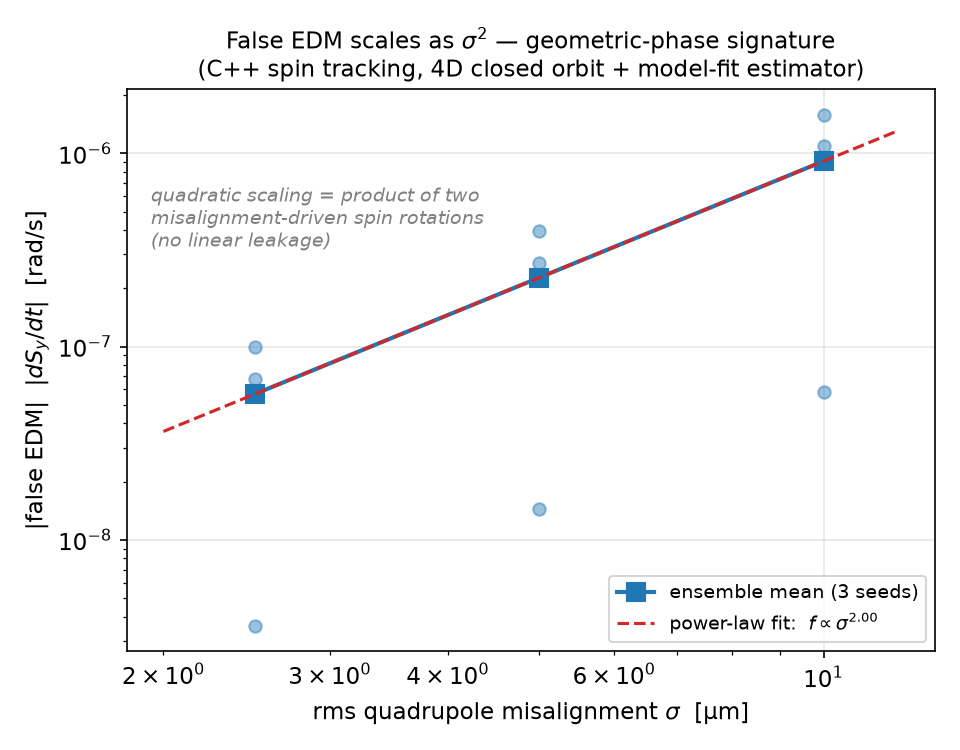
\includegraphics[width=\columnwidth]{fig_orbit_sigma.png}
\caption{Validation of the false-EDM estimator: the measured $|dS_y/dt|$ scales
as $\sigma^{2.00}$ across $\sigma = 2.5$--$10~\mu$m (C++ tracking, three seeds
per point) --- the fingerprint of a pure geometric phase with no linear
leakage.  The scatter between seeds reflects that $f$ is a product $dx\cdot dy$:
individual patterns can happen to be small.}
\label{fig:sigma}
\end{figure}

\begin{figure*}[tb]
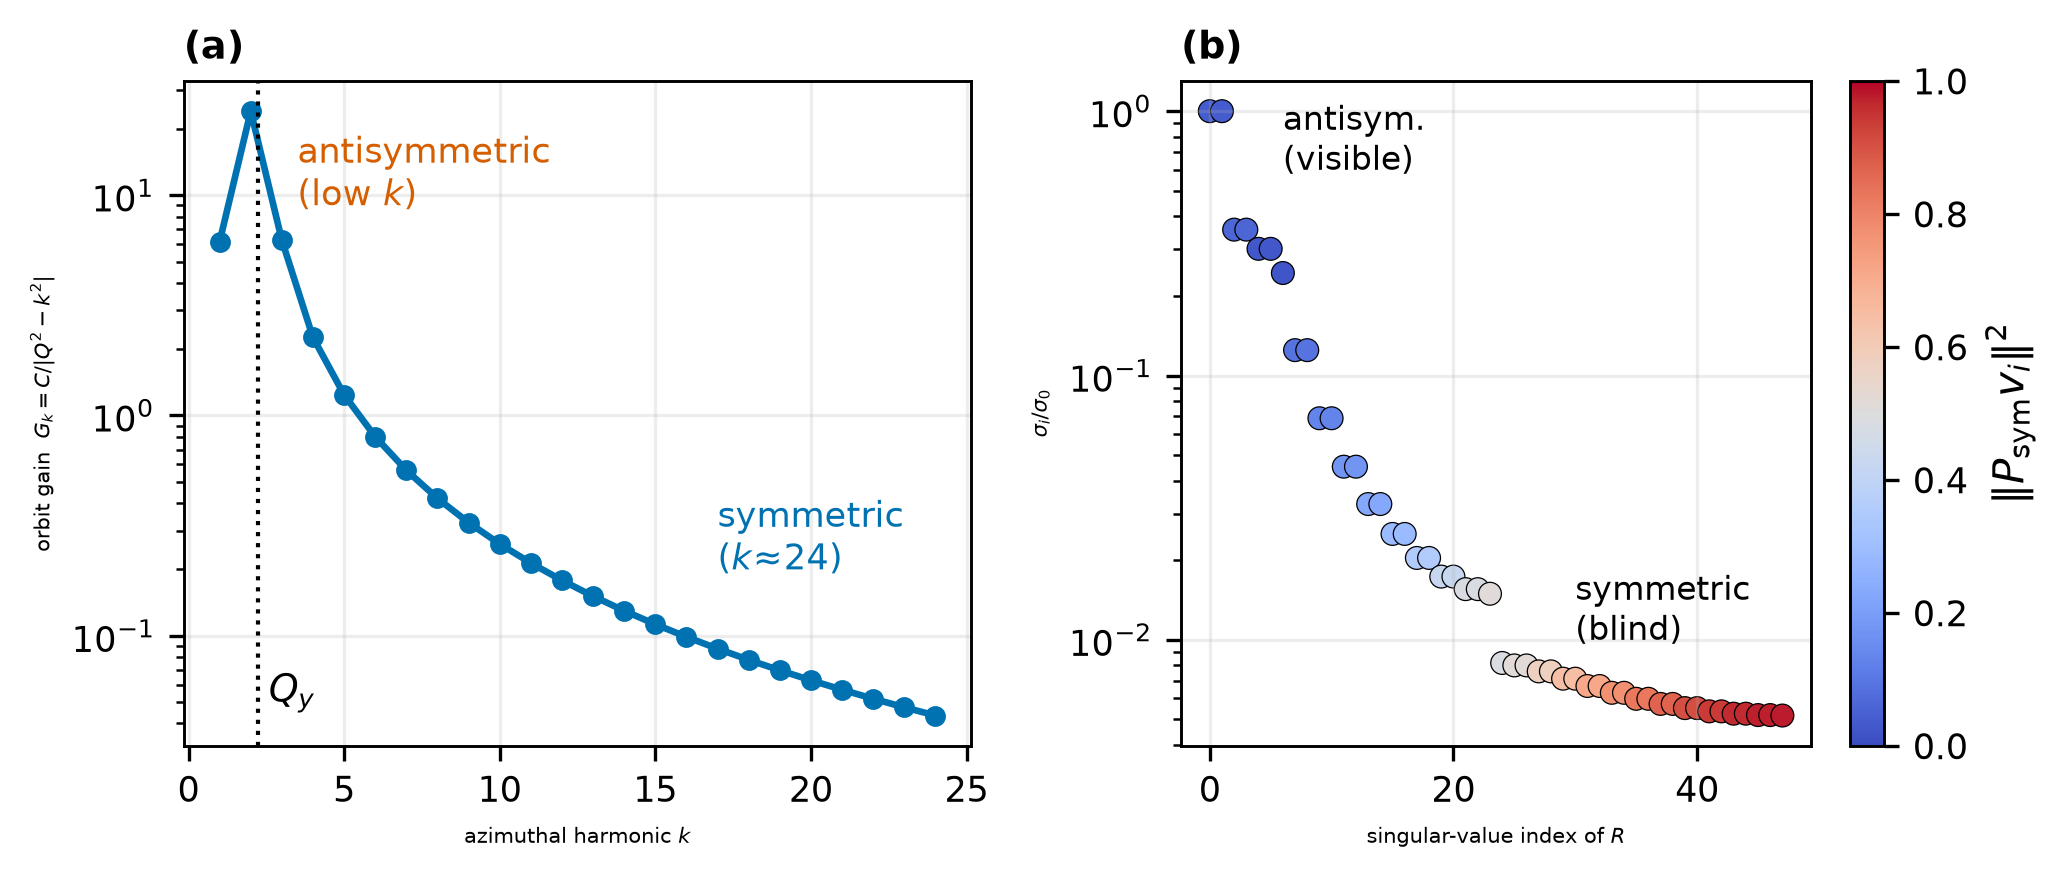
\includegraphics[width=0.95\textwidth]{fig_orbit_modes.png}
\caption{Mode structure of the orbit response (analytic lattice,
$Q_y = 2.30$).  Left: singular values of $R$, colored by how symmetric the
corresponding misalignment mode is; the visible modes are antisymmetric, the
invisible ones symmetric; $\mathrm{cond}(R)=193$.  Right: the orbit gain law
$G_k = C/|Q^2-k^2|$; antisymmetric patterns give low-$k$ kicks near the
resonance, symmetric patterns give $k\approx24$ kicks far above it.}
\label{fig:modes}
\end{figure*}

\subsection{How we score a reconstruction: the correlation trap}
\label{sec:metrics}

We use two scores, and the difference between them decides several results, so
we state both.

\paragraph{Pearson correlation --- the misleading one.}
Between a reconstruction $\hat v$ and the truth $v$ over 48 components,
$\mathrm{corr}$ is the usual normalized dot product.  It misleads here for two
reasons.  First, it subtracts the mean, which removes exactly the worst (uniform)
member of the symmetric family from the error.  Second, it is dominated by the
many well-reconstructed antisymmetric components.  As a result,
\emph{$\mathrm{corr}=0.99$ can coexist with a completely wrong symmetric
component} (Fig.~\ref{fig:lockin} shows a case).

\paragraph{Component error --- the honest one.}
The rms, \emph{without} subtracting the mean, of the symmetric and antisymmetric
parts of the error $e = \hat v - v$, compared against the corresponding parts of
the signal itself (both $\approx 41~\mu$m for $\pm100~\mu$m uniform
misalignments).  A method truly ``sees'' the symmetric component only if its
symmetric error is below the symmetric signal.

\subsection{Systematic-error models}
\label{sec:systematics}

Four systematics enter at realistic sizes:

\begin{itemize}
\item \textbf{BPM offsets} (static, $\sim\!100~\mu$m each; $30~\mu$m variant):
each monitor's electronic zero differs from the true axis by an unknown but
steady constant.  The main killer of single-orbit inversion; it cancels in any
difference measurement (like $K$-modulation or drift monitoring).
\item \textbf{BPM noise} (random, $\sim\!1~\mu$m per shot): averages down as
$\sqrt{N}$, so with synchronous detection it stops being a practical limit.  A
central message of this paper is that the real limit is \emph{not} this.
\item \textbf{BPM gain errors} (multiplicative, $1$--$10\%$): percent-level
scale errors of the readings; partly softened by averaging over BPMs.
\item \textbf{$\beta$-beating / model error} (per-quadrupole $0.5$--$5\%$,
applied in the tracker as small gradient deviations): the gap between the real
optics and the model used to analyze the data (a LOCO-calibrated machine
typically leaves $\sim\!1\%$).  This is \emph{coherent} --- it does not average
down --- and it turns out to be the decisive wall.
\item \textbf{Quadrupole tilt} (roll angle $\psi$): two channels, cross-plane
leakage into the measurement and a direct geometric-phase term in the false EDM;
the latter dominates and is reported as its own tolerance.
\end{itemize}

\paragraph{Seed policy.}
Because $f$ is a product, it can be accidentally small or large for one
misalignment draw, so every claim is averaged over many realizations (typically
3--40) and no conclusion is drawn from a single seed.

% ═══════════════════════════════════════════════════════════════════
\section{Simulation results}
\label{sec:results}

\subsection{What orbit control does deliver}
\label{sec:chain}

Start with what works.  For $\sigma = 10~\mu$m misalignments in both planes the
raw false EDM is $|f| \approx 10^{-6}$~rad/s, about $1000\times$ target
[Eq.~(\ref{eq:target})].  Two standard steps cut it down
(Table~\ref{tab:chain}, Fig.~\ref{fig:suppression}):

\begin{enumerate}
\item \emph{Run both beams at once.}  The real EDM flips sign when the beam
direction reverses [Eq.~(C1) of \cite{omarov}], so the CW/CCW difference cancels
the part of the false EDM that does \emph{not} flip.  Measured gain: $3.4\times$
(ensemble median), leaving $474\times$ target.
\item \emph{Correct the orbit.}  Flattening the orbit with correctors removes
the visible (antisymmetric) part of the misalignment imprint.  Measured extra
gain: $7.7\times$, leaving $\bm{62\times}$ \textbf{target}
($6.05\times10^{-8}$~rad/s $\approx 6\times10^{-28}\,e\!\cdot\!$cm).
\end{enumerate}

What is left after both steps sits almost entirely in the symmetric,
orbit-blind pattern of Sec.~\ref{sec:symanti}, and by Eq.~(\ref{eq:sigma2}) it
scales as $\sigma^2$.  The central deliverable of the paper is therefore the
curve of Fig.~\ref{fig:suppression}.  To reach the target along it, the
\emph{symmetric} misalignment must be at or below
$\sigma_{\rm sym} \approx 1.3~\mu$m.  Two facts make that hard.  First, as the
rest of this section shows, no orbit measurement can verify it.  Second, a tape
measure cannot verify it either, because what matters is the \emph{magnetic}
center: stray fields at the $\sim\!20~\mu$T level move the magnetic center tens
of microns away from the mechanical one, and only the beam sees the magnetic
center.

\begin{table}[tb]
\caption{The suppression chain at $\sigma = 10~\mu$m (C++ tracking).  The
equivalent EDM uses $1~\text{nrad/s} \leftrightarrow 10^{-29}\,e\!\cdot\!$cm.}
\label{tab:chain}
\begin{ruledtabular}
\begin{tabular}{lcc}
Stage & $|f|$ / target & equiv.\ EDM [$e\!\cdot\!$cm] \\
\hline
raw (no correction)          & $\sim1000\times$ & $\sim10^{-26}$ \\
$+$ CW/CCW difference        & $474\times$      & $\sim5\times10^{-27}$ \\
$+$ orbit correction         & $62\times$       & $\sim6\times10^{-28}$ \\
$+$ any method of Sec.~\ref{sec:inverse} & $62\times$ & floor \\
\end{tabular}
\end{ruledtabular}
\end{table}

\begin{figure}[tb]
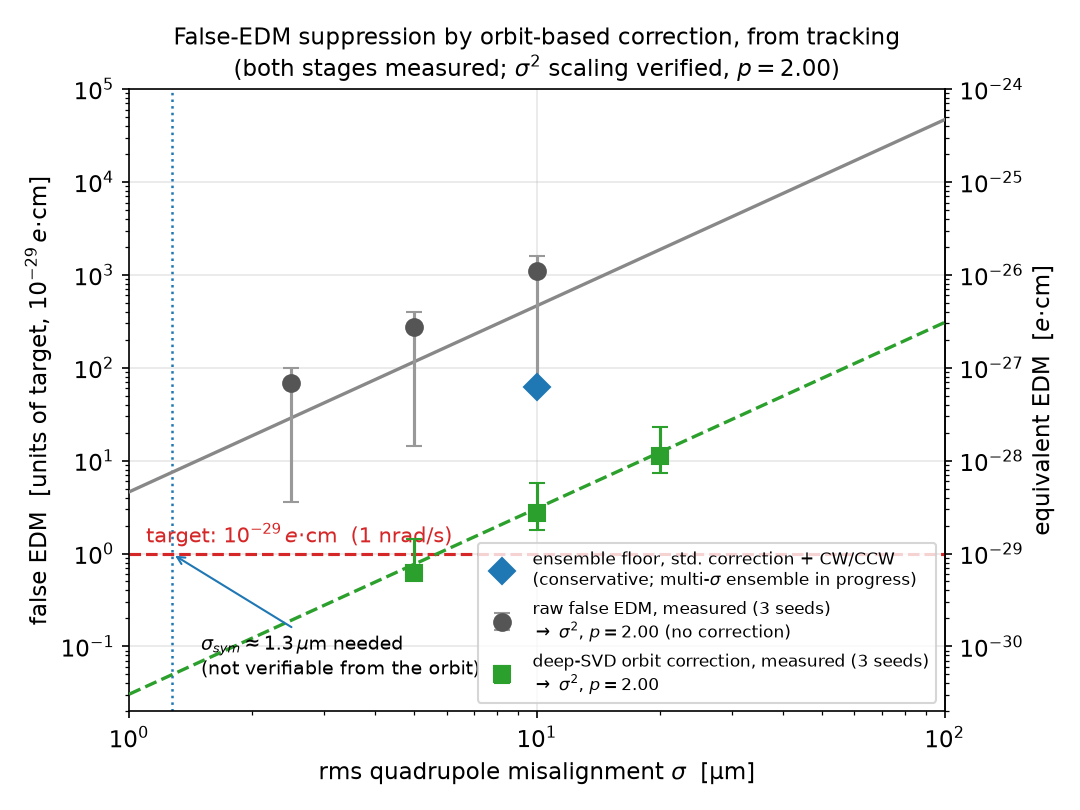
\includegraphics[width=\columnwidth]{fig_orbit_suppression.png}
\caption{Main result: the false EDM reachable by orbit correction versus the rms
quadrupole misalignment.  The points at $\sigma=10~\mu$m are C++ tracking; all
curves scale as $\sigma^2$ ($p=2.00$).  The corrected floor crosses the target
only at $\sigma_{\rm sym}\approx1.3~\mu$m --- a level no orbit measurement can
verify.}
\label{fig:suppression}
\end{figure}

\subsection{Trying to measure the hidden component from the orbit}
\label{sec:inverse}

Everything in this subsection shares one idea: reconstruct the misalignments
(or their symmetric part) from orbit readings, then correct.  Five independent
attempts hit the same wall.

\subsubsection{Common-frequency $K$-modulation with matrix inversion}
\label{sec:deltaR}

Modulate all quadrupole gradients together between two settings ($g$ and
$1.02g$) and subtract the two orbits.  The static BPM offsets cancel exactly,
leaving $\Delta y = \Delta R\,\Delta q$ with $\Delta R = R(1.02g) - R(g)$.  With
no errors, inverting this $48\times48$ matrix recovers the offsets perfectly
($\mathrm{corr}=1.000000$), and optics breathing (below) is not a problem here
because it is already contained in $\Delta R$.  The problem is conditioning:
$\mathrm{cond}(\Delta R) = 3.7\times10^{4}$ with
$\sigma_{\min} \approx 10^{-4}$, and the weak directions are the symmetric ones.

Random BPM noise \emph{can} be beaten: modulating at $\sim\!1$~kHz with lock-in
(synchronous) detection averages the noise down as $\sqrt{N}$, reaching
$\sim\!14$~nm in about 17~minutes.  The limits that remain are the ones that do
not average [Fig.~\ref{fig:lockin}].  Even at a 10~nm noise floor with a
\emph{perfect} optics model, the symmetric error is already a third of the
symmetric signal.  With a realistic model error the inversion collapses:
$\varepsilon = 0.5\%$ of $\beta$-beating drives the symmetric error to
$\sim\!7\times$ the signal (283~$\mu$m vs.\ 41~$\mu$m), while the correlation
still reads a reassuring $0.69$.  Because $\beta$-beating is coherent, no BPM
technology --- including SQUID BPMs, whose low noise would only shorten the
integration time --- changes this floor.

\begin{figure}[tb]
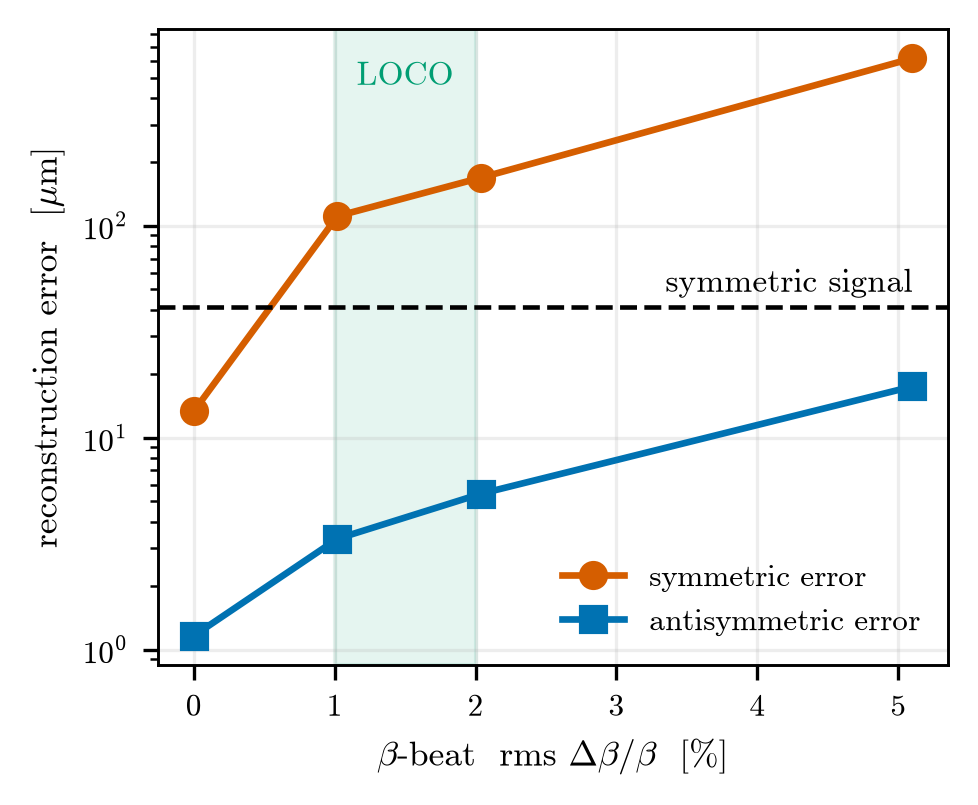
\includegraphics[width=\columnwidth]{fig_orbit_lockin.png}
\caption{Single-frequency $\Delta R$ inversion at the lock-in noise floor
(10~nm, 40 seeds).  Symmetric and antisymmetric reconstruction errors versus the
optics-model error $\sigma_g$; the dashed line is the symmetric signal itself.
Any realistic model error ($\geq0.5\%$) pushes the symmetric error far above the
signal while the correlation (gray labels) stays deceptively high --- the
correlation trap of Sec.~\ref{sec:metrics}.}
\label{fig:lockin}
\end{figure}

\paragraph{A lower bound behind this.}
This is not an accident of the scheme.  Cancelling the static offsets by any
two-setting difference means the useful information is no longer $R$ but
$\Delta R \sim \varepsilon_g\,\partial R/\partial g$, whose inverse grows as
$\|\Delta R^{-1}\| \sim \|R^{-1}\|/\varepsilon_g$.  So within the natural class
of linear, unbiased estimators that cancel offsets by a two-setting difference,
offset immunity is bought at the price of a $1/\varepsilon_g$ noise blow-up.  We
state this as a structural lower bound for that class; estimators outside it
(e.g., Bayesian modeling of the offsets) are not covered.

\subsubsection{Per-quadrupole modulation read as an amplitude: optics breathing}
\label{sec:breathing}

A seemingly stronger idea drops matrix inversion.  Modulate each quadrupole at
its \emph{own} frequency ($\sim\!2\%$ depth); the strength $A_i$ of frequency
$f_i$ in a BPM signal should be proportional to that magnet's beam offset $o_i$,
giving a direct per-magnet readout --- the ac-BBA idea of Ref.~\cite{marti}
moved to this ring.  Because the modulation ($1$--$10$~kHz) is far below the
betatron frequency ($\sim\!515$~kHz), the beam follows the slow change and each
amplitude equals a static derivative $\partial y_{\rm BPM}/\partial g_i$.

It fails for a reason worth understanding [Fig.~\ref{fig:breathing}].  Wiggling
quadrupole $i$'s strength does two things: it modulates that magnet's own kick
(the signal we want, $\sim\!0.9~\mu$m at the BPM), and it modulates the optics
everywhere --- $\beta(s)$, $\phi(s)$, and $Q$.  The pre-existing orbit
($\sim\!0.37$~mm rms, built by all 48 offsets together) is re-transported
through this slightly-changed optics, giving a few-$\mu$m response at the BPM:
the optics ``breathes.''  Breathing beats signal by about $7$ to $1$.  A clean
decomposition makes the point: the response to modulating one quadrupole is
$-9.83~\mu$m with the full pattern present, but only $-0.037~\mu$m when only
that magnet's own offset is kept --- a factor $266$.  The measured amplitude
reads \emph{the orbit built by the neighbors}, not the magnet's own offset, so
dividing by a calibration is meaningless.

Because breathing is coherent (roughly the existing orbit times a number), it
does not average away: going from 1 to 48 BPMs leaves the correlation at zero
($+0.07 \to -0.03$), and a SQUID's low noise does not help, because noise was
never the problem.  Remove the breathing in an idealization and the same
pipeline reconstructs perfectly ($\mathrm{corr}=1.000$), pinning the blame
squarely on breathing.  The C++ tracker confirms the analytic breathing
amplitudes to $\sim\!1\%$.  BPM offsets are irrelevant in this branch ---
ac demodulation removes the static offset --- so improving offsets from 100 to
$30~\mu$m changes nothing.

The two $K$-modulation failures are conceptually different: breathing is a
coherent \emph{contamination} that kills the per-magnet readout, while
conditioning is a \emph{noise blow-up} of the inversion.  Different walls, and
each closes its branch.

\begin{figure*}[tb]
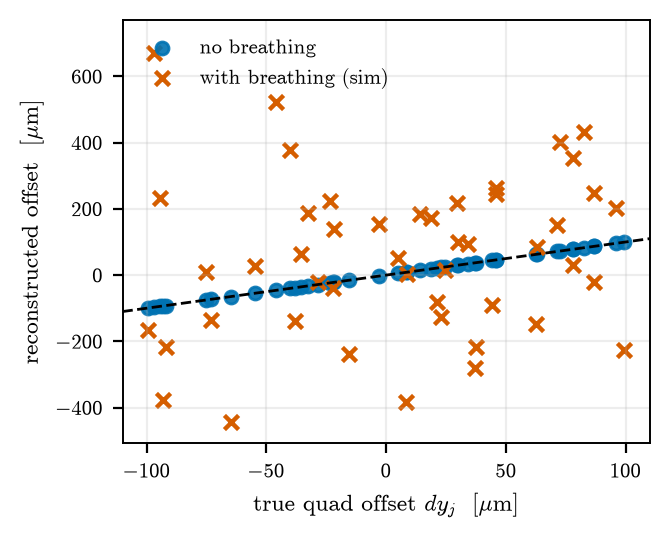
\includegraphics[width=0.95\textwidth]{fig_orbit_breathing.png}
\caption{Distributed-frequency per-quadrupole modulation.  Left: reconstructed
vs.\ true offsets --- perfect without breathing (green), zero correlation with
breathing, for 1 BPM (red) and even 48 BPMs (purple).  Right: the ``lever'' ---
the demodulated amplitude responds to the whole pre-existing orbit ($266\times$
the magnet's own contribution); being coherent, this contamination does not
average away with more BPMs or a better (SQUID) resolution.}
\label{fig:breathing}
\end{figure*}

\subsubsection{Neural-network reconstruction}
\label{sec:nn}

Could a trained network beat the linear algebra?  No, and the reason is
instructive.  The map misalignment~$\to$~orbit is \emph{exactly linear}
($y = R\,\Delta q$), so a network trained on it can only relearn $R$; inverting
is then $R^{-1}$ with the same conditioning.  In numbers, a multilayer
perceptron (two hidden layers of 128, 4000 samples, 1~$\mu$m BPM noise)
reconstructs the antisymmetric part as well as truncated SVD (0.71 vs.\
0.63~$\mu$m error) and fails on the symmetric part just as badly (5.6 vs.\
6.3~$\mu$m error against a 9.9~$\mu$m signal).  The limit is
information-theoretic: the symmetric imprint is below the noise-plus-systematics
floor, and no estimator can pull out information that is not in the data.  For
the same reason fancier architectures cannot help --- capacity is not the
bottleneck in a linear problem --- and for random noise the lock-in filter is
already optimal, so learned time-series models cannot beat it either.  Any real
gain would need \emph{prior information}; sparsity priors (LASSO, CLEAN, greedy
harmonic selection) were tried and hit the same floor.

\subsubsection{Calibrate once, then monitor drift (LOCO)}
\label{sec:drift}

A pragmatic approach gives up on absolute alignment and asks only for its
\emph{changes}: calibrate the machine once (LOCO), then watch the orbit
difference $y(t) - y_0$, in which the static offsets cancel.  This works well
for what it sees: drifts are tracked to $6.5~\mu$m rms under $50~\mu$m BPM
offsets (a $29\times$ gain over absolute reconstruction), degrading only mildly
with $1\%$ $\beta$-beating.  But the difference orbit still passes through the
same response matrix: its eight worst modes are $96\%$ symmetric with a
$193\times$ noise blow-up.  The drift monitor is a cheap, useful watchdog for
the antisymmetric part --- and blind to the symmetric part, like everything else
in this class.

\subsubsection{Harmonic approaches}
\label{sec:harmonic}

Two harmonic variants deserve a note.  \emph{Targeted Fourier reconstruction:}
if the harmonic content of the misalignment is known ahead of time, restricting
the basis improves the conditioning from $\sim\!13000$ to 186 and it works; but
for unknown patterns, greedy or LASSO harmonic selection collapses from rank
deficiency --- knowing \emph{which} harmonics is exactly the missing
information.  \emph{Fit of a known signature:} reading a known field imprint
(e.g., an $N{=}2$ stray radial field, which drives a $k{=}2$ vertical orbit) by
projecting the 48-BPM data onto $\cos2\theta/\sin2\theta$ is perfectly
conditioned but \emph{biased}: the one $k{=}2$ number lumps together the field,
the misalignment's $k{=}2$ content, and the BPM offsets' $k{=}2$ content --- a
$\sim\!53$~nT bias at $10~\mu$m against a 1~nT target here.  Full regularized
SVD does not beat it under realistic offsets: its detection floor is
$\sim\!45$~nT at $100~\mu$m offsets (2.6~nT only for ideal, offset-free BPMs).
In the language of Ref.~\cite{wegscheider}, the forward projection is
bias-limited, the inversion is noise-limited, and neither reaches the degenerate
information.

\subsubsection{The counter-rotating beam separation}
\label{sec:crsep}

Reference~\cite{omarov} proposes controlling the geometric phase by measuring
and zeroing the \emph{separation} between the CW and CCW orbits.  But the
separation is itself an orbit difference, so it inherits the orbit's mode
structure.  We measured this directly [Fig.~\ref{fig:crsep}]: for $10$-$\mu$m
vertical patterns the ratio of antisymmetric to symmetric signature is
$5.7\times$ in a single-beam orbit and $8.0\times$ in the CR separation (three
seeds; an independent set gave $3.8\times$ and $4.5\times$).  The suppression is
similar, so \emph{the CR separation opens no extra window on the symmetric
part}.  Measuring and zeroing it controls the visible part of the geometric
phase --- consistent with Ref.~\cite{omarov} --- and leaves the symmetric
residual of Table~\ref{tab:chain} untouched.  This closes gap~(ii) of the
Introduction.

\begin{figure}[tb]
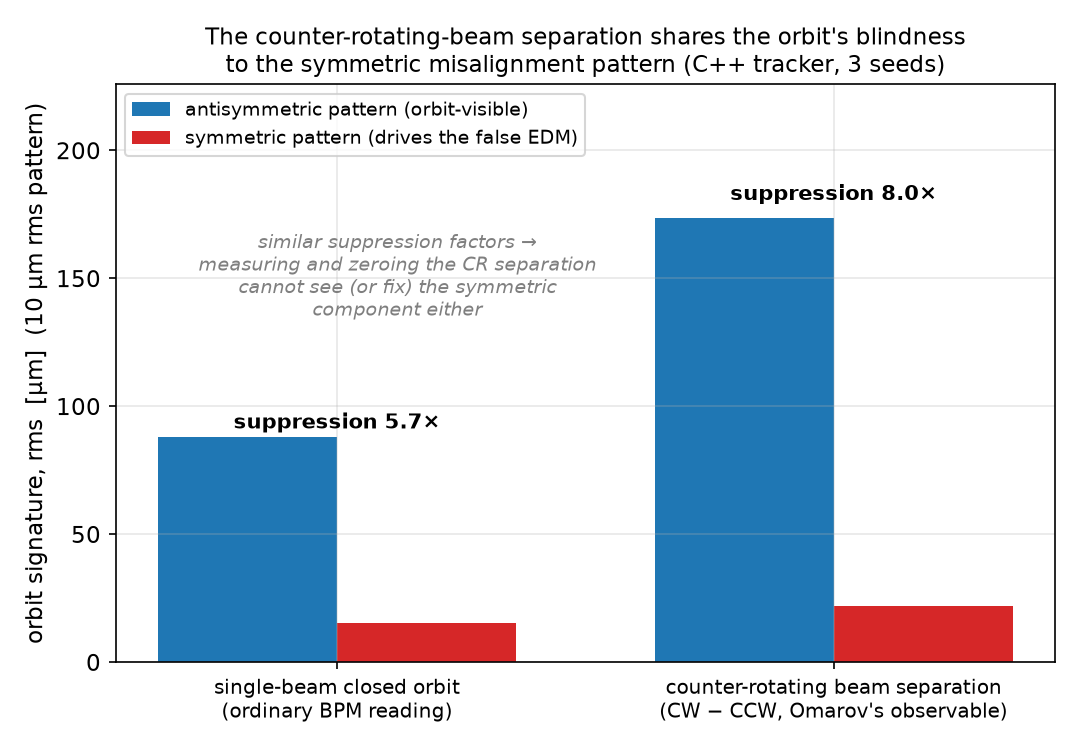
\includegraphics[width=\columnwidth]{fig_orbit_crsep.png}
\caption{The counter-rotating beam separation (right group) suppresses the
symmetric pattern by about the same factor as the ordinary single-beam orbit
(left group): the control observable of Ref.~\cite{omarov} shares the orbit's
blindness to the component that drives the residual false EDM.}
\label{fig:crsep}
\end{figure}

\subsection{Trying to open the symmetric window at the lattice level}
\label{sec:escape}

Two lattice-level escapes were examined.

\subsubsection{Quadrupole polarity switching}
\label{sec:flip}

Reversing all quadrupole currents ($g \to -g$) reverses each
misalignment-driven spin rotation, so one might hope it flips the false EDM
while leaving the real (electric-field-driven) EDM alone.  It does not.  The
geometric phase is a \emph{product of two} field-driven rotations, each
$\propto g$, so $f$ is \emph{even} in $g$.  Measured flip ratios $f(-g)/f(+g)$
are $+2.8$, $+0.85$, and $+1.17$ for symmetric, antisymmetric, and generic
patterns --- the sign never reverses.  Moreover, in the idealized periodic
lattice the polarity flip is \emph{degenerate} with reversing the beam:
$f({\rm CCW}, +g) = f({\rm CW}, -g)$ to a measured $1.00$, so the four-way
combination of Eq.~(C2) of Ref.~\cite{omarov} collapses to the two-way CW/CCW
difference, and polarity switching gives no independent cancellation for the
geometric phase.  (It stays useful against systematics that are odd in $g$.)
This closes gap~(iii) of the Introduction.

\subsubsection{Raising the betatron tune}
\label{sec:highQ}

The symmetric pattern is hidden because its kick harmonic ($k \approx 24$) sits
far above the tune [Eq.~(\ref{eq:Gk})]; raising $Q$ toward $k$ should make it
visible.  It partly does: at $Q_y \approx 10.3$ (still alternating focusing,
still stable) the high-harmonic part of the symmetric family reaches orbit gains
like the antisymmetric ones.  But the low-harmonic part needs $Q \geq 16$, while
the $180^\circ$-per-cell stopband caps the tune at $Q \leq 12$; only
$\sim$8--25\% of the symmetric content becomes recoverable, worth only a
factor $\sim\!2$ in false-EDM suppression.

More decisively, a high tune needs \emph{strong quadrupoles}:
$Q_y\!: 2.3 \to 10.3$ needs $g\!: 0.21 \to 0.69$~T/m.  Stronger gradients kick
the beam harder for the same misalignment; since the geometric phase is a
product of two such rotations ($\propto g^2$), plus a term from the larger
betatron orbit, the false EDM grows steeply --- a single-pattern C++ run gave a
factor $\sim\!32$ ($\sim g^3$) from $g = 0.21$ to $0.69$~T/m --- while the real
EDM, driven by the electric field, is independent of $g$.  So the
signal-to-background \emph{worsens} by that same large factor: one cannot
operate at high tune, and a brief high-tune diagnostic transfers at most the
recoverable $\sim$25\% back to the operating point.  (At $Q\approx10$ the
closed-orbit determination itself becomes delicate; our scans at $g=0.69$~T/m
carried residual-betatron contamination, so we quote only the robust
qualitative conclusion and the single clean pattern above.)

\subsection{The one technique that escapes the wall: null-finding BBA}
\label{sec:bba}

All the walls above come from either inverting a response matrix or dividing a
demodulated amplitude by a calibration.  Standard quadrupole beam-based
alignment (BBA) does neither.  It steers the beam through each quadrupole and
finds the magnetic center as the beam position where the response to a
gradient change \emph{vanishes} --- a zero-crossing.  A zero-crossing does not
depend on how big the response is, so it is not amplified by the conditioning,
and it is transparent to $\beta$-beating in ideal optics.  It carries no
``symmetric blindness.''

\paragraph{How the measurement works, step by step.}
The procedure is the standard one, applied to each of the 47 alignable
quadrupoles in turn (the special modulated quadrupole of cell 0 is excluded, so
its offset is set to zero and reported).  To find the center of quadrupole $i$:
\begin{enumerate}
\item \emph{Steer the beam across it.}  Using the nearest corrector, scaled by
the single response-matrix element $R_{ij}$ so that the applied setting moves the
beam by a chosen amount ($\sim\!150~\mu$m) at quadrupole $i$, place the beam at
two positions bracketing the expected center.
\item \emph{Modulate the gradient.}  At each of the two beam positions, change
quadrupole $i$'s gradient by a small step $\delta g$ and record the difference of
the closed orbits, ``on'' minus ``off,'' at all 48 BPMs.  This orbit difference
is the imprint of a thin lens of strength $\delta g$ placed at the beam's offset
from the magnetic center, so it is proportional to that offset.
\item \emph{Find the zero-crossing.}  Because the imprint is proportional to the
offset, it changes sign as the beam crosses the center.  From the two bracketing
positions the center is the offset where every BPM's imprint would vanish; we
take the least-squares zero over the 48 BPMs, weighting each by how strongly it
responds.  The spread of the individual BPM zero-crossings is a built-in
quality flag for that magnet.
\end{enumerate}
Every closed orbit in steps~1--2 is read with the tracked particle sitting on the
4D closed orbit (Sec.~\ref{sec:estimator}), so the reading is free of the
betatron artifact.  The 47 centers found this way \emph{are} the misalignments;
subtracting them from the corrector pattern flattens the orbit.

\paragraph{Why the response matrix appears here, yet the blindness does not.}
It is fair to ask how this method can lean on the \emph{same} response matrix $R$
whose inversion failed in Sec.~\ref{sec:inverse}.  The answer is that BBA never
inverts $R$.  The inversion methods ask one \emph{global} question --- given the
whole orbit, which 48-component misalignment produced it? --- and the symmetric
pattern lies almost in the null space of $R$, so answering it means dividing by
the tiny symmetric singular values and amplifying every error by
$\mathrm{cond}(R)=193$.  BBA instead asks 47 \emph{local} questions --- where is
the center of this one magnet? --- each answered by a direct zero-crossing of the
beam, with no global inverse anywhere.  The response matrix enters only in the
\emph{forward} direction, and only through the single well-conditioned element
$R_{ij}$ that sizes the steering bump; it positions the ruler, it is not the
quantity solved for.  The symmetric-versus-antisymmetric distinction exists only
in the 48-vector of \emph{answers}, and BBA measures every component of that
vector directly and equally well, so it has no preferential blindness to the
symmetric combination.  This same picture explains the horizontal stall: a wrong
forward element $R_{ij}$ --- the deflector-as-drift error above --- mis-sizes the
bump and shifts the reading, but it does not bring back the symmetric null space.
It is a separate, local, and fixable error, not a return of the wall.

\paragraph{Idealized optics: it works.}
In clean optics, null-finding BBA measures the symmetric centers and cuts the
false EDM from $\sim\!356\times$ to $\sim\!1.6\times$ target --- the wall of
Sec.~\ref{sec:inverse} is genuinely absent for this method.

\paragraph{Realistic optics: breathing hits here too.}
Under $1\%$ $\beta$-beating a single pass fails, for a familiar reason.  To
steer the beam through one magnet we build a local orbit bump, and modulating
that magnet re-transports the large uncorrected orbit through the beating optics
(the same breathing as Sec.~\ref{sec:breathing}), biasing the zero-crossing.
The cure is the natural one: correct the orbit first so it is small, then repeat
--- ``align, flatten, re-align.''  Each pass shrinks the orbit, so each pass
breathes less.

\paragraph{Why vertical works and horizontal stalls: a testable diagnosis.}
Before giving the numbers we state, and then test, the cause of the difference
between the two planes.  It is not a law of physics; it is a limitation of the
\emph{model we steer with}.  The local bumps are built from an optics model, and
the fast analytic solver of Sec.~\ref{sec:method} treats the electric deflectors
as field-free drifts.  In the vertical plane that is nearly exact --- the ring's
radial deflector field barely focuses vertically --- so the model matches the
machine and the bumps land where intended.  The horizontal plane is the plane the
ring bends in, and there the deflectors do two things the model omits: they focus
the beam horizontally, and they bend it, which creates dispersion.  A one-line
check exposes the gap.  Treating the deflectors as drifts, the model predicts
\emph{identical} tunes in the two planes, $Q_x = Q_y = 2.303$.  The real ring
matches this vertically to four decimals ($0.3032$ measured vs.\ $0.3032$) but
its horizontal tune is higher by $0.052$ in fractional part --- the deflector
focusing the model leaves out.  A direct comparison of the response matrices is
even starker: element by element the measured horizontal response is essentially
uncorrelated with the analytic one (median ratio near zero, often opposite sign),
so the analytic model picks the \emph{wrong} steering corrector for 36 of the 47
magnets, whereas vertically it agrees to $5\%$ and picks the wrong corrector only
12 times.  A wrong corrector means the beam is scanned across the wrong range and
the zero-crossing is biased.  The diagnosis therefore predicts a concrete fix:
steer with the \emph{measured} response matrix, not the idealized one.

\paragraph{Testing the fix: idealized vs.\ measured steering.}
We ran the full iteration two ways, identical but for the steering matrix ---
the idealized analytic model, and the ring's measured response matrix (obtained
by displacing each magnet in the tracker and recording the orbit)
--- both under $1\%$ $\beta$-beating, three passes
(Table~\ref{tab:bba}).  Both solve the \emph{vertical} plane identically: the
orbit shrinks $48\to9~\mu$m and the vertical symmetric residual halves each pass
($3.3\to1.7\to0.9~\mu$m).  They differ sharply in the \emph{horizontal} plane.
With the idealized model the horizontal magnets never really correct (the first
pass is even worse than no correction) and the false EDM bottoms out at
$145\times$ target.  With the measured matrix the horizontal magnets correct too:
the false EDM falls to $17\times$ target by the second pass --- nine times lower
--- and the horizontal residual drops from $4.3$ to $2.3~\mu$m.  This confirms
the diagnosis directly: the horizontal stall was a fault of the steering model,
not of the method.

Two honest caveats remain.  First, the measured-matrix run is
\emph{non-monotonic}: the third pass ($28\times$) is worse than the second
($17\times$).  Because the false EDM is a product $dx\cdot dy$ and the horizontal
residual is still a few times larger than the vertical, the bilinear value
bounces as the residual pattern shifts from pass to pass; the procedure should be
stopped at its best pass rather than run open-loop.  Second, it does not reach the
target: the best floor is $\sim\!17\times$ ($\approx2\times10^{-28}\,e\!\cdot\!$cm),
still an order of magnitude high.  The horizontal plane is much improved but still
trails the vertical, plausibly because the response matrix here was measured on
the ideal lattice while the run carries $\beta$-beating (on a real machine one
would measure it on the actual, beating machine), and because residual breathing
and dispersion still bias the reading.  Closing this last gap, and the hardware
floor below, is the remaining work.

\begin{table}[tb]
\caption{Iterated null-finding BBA under $1\%$ $\beta$-beating (C++ tracking,
three passes), steering with the idealized analytic model vs.\ the measured
response matrix.  ``sym $dx$/$dy$'' are the symmetric-component residuals
[Eq.~(\ref{eq:projectors})] of the measured-matrix run.  Both solve the vertical
plane; only the measured matrix also corrects the horizontal one, lowering the
false-EDM floor by about nine.}
\label{tab:bba}
\begin{ruledtabular}
\begin{tabular}{lcccc}
     & sym $dy$ & sym $dx$ & \multicolumn{2}{c}{$|f|$ / target} \\
pass & [$\mu$m] & [$\mu$m] & analytic & measured \\
\hline
raw  & ---  & ---  & $356\times$ & $356\times$ \\
1    & 3.27 & 4.27 & $368\times$ & $73\times$ \\
2    & 1.70 & 2.90 & $238\times$ & $\bm{17\times}$ \\
3    & 0.91 & 2.29 & $145\times$ & $28\times$ \\
\end{tabular}
\end{ruledtabular}
\end{table}

\paragraph{On the stabilizing knobs.}
The iteration carries two settings: how aggressively each correction is applied
(under-relaxation), and a quality cut that throttles magnets whose zero-crossing
is inconsistent across BPMs.  With the idealized steering these merely prevent the
horizontal plane from diverging (without them its residual blows up to
$\sim\!12~\mu$m) without curing it --- stability, not a solution.  With the
measured steering the horizontal magnets are consistent enough that the quality
cut stops throttling them (its minimum horizontal quality rises from $0$ to
$0.3$ across the passes), which is why the plane finally corrects.  The knobs
buy robustness; the physics fix is the correct steering matrix.

\paragraph{Summary of the method.}
Null-finding BBA is the one measurement class not excluded by the walls of
Sec.~\ref{sec:inverse}.  In clean optics it recovers the symmetric component
outright.  Under realistic $\beta$-beating it solves the vertical plane cleanly,
and --- once steered with the measured rather than the idealized response matrix
--- it also corrects the horizontal plane, lowering the false-EDM floor by about
nine (to $\sim\!17\times$ target).  The horizontal plane still trails the
vertical and the floor is an order of magnitude above the goal, so we present
null-finding BBA as the promising route with a demonstrated, physics-based fix
for its main obstacle, not yet as a finished solution: closing the residual
horizontal gap (measuring the response on the $\beta$-beating machine, stopping
at the best pass) and the hardware floor below remain to be done.

\subsection{Outside the orbit: off-momentum spin sensing (brief)}
\label{sec:offmomentum}

For completeness we record one attempted escape outside the orbit toolbox.
Storing the beam slightly off the magic momentum makes the in-plane spin precess
at $\nu_s \neq 0$, and the geometric-phase part of the vertical oscillation is
indeed \emph{amplified} $\propto 1/\nu_s$ --- suggesting a fast, resonant
readout.  It fails because misalignments also tilt the invariant spin axis at
\emph{first} order in $\sigma$: this $\mathcal{O}(\sigma)$ oscillation sits at
the same frequency $\nu_s$ and beats the $\mathcal{O}(\sigma^2)$ geometric term
by $\sim\!3600$ at $\sigma=10~\mu$m.  Every way to separate the two was tested
and closed: they do not separate in $\delta p/p$, their relative phase is
pattern-dependent, four-fold sampling does not cancel the first-order term (it
is common to the four particles), the amplitude crossing lies at an unphysical
$\sigma \approx 62$~mm, a full 3D fit of the invariant axis leaves no residual,
and the longitudinal component is knob-insensitive off-magic.  The magic
momentum is the \emph{unique} working point that turns the dominant first-order
effect into a harmless constant offset --- which is also why the estimator of
Sec.~\ref{sec:estimator} works there.

% ═══════════════════════════════════════════════════════════════════
\section{Conclusions}
\label{sec:conclusions}

\paragraph{Quantitative result.}
The orbit-based chain --- both beams at once, standard orbit correction, and
continuous drift monitoring --- bounds the quadrupole-misalignment false EDM at
$\sim\!6\times10^{-28}\,e\!\cdot\!$cm for $\sigma = 10~\mu$m, and the bound
scales as $\sigma^2$ (Fig.~\ref{fig:suppression}).  If the required suppression
were only to $10^{-27}\,e\!\cdot\!$cm, existing BBA technology would suffice.
Reaching $10^{-29}\,e\!\cdot\!$cm needs the \emph{symmetric} part of the
magnetic-center misalignment held near $1.3~\mu$m.

\paragraph{Wall for the response-matrix and amplitude classes.}
The symmetric component is unobservable at the required level in every channel
of these classes we tested: common-frequency $K$-modulation with (regularized)
inversion, per-quadrupole modulation read as an amplitude, neural networks,
LOCO-plus-drift monitoring, harmonic fits, and the counter-rotating beam
separation.  For all of them the limit is set not by random BPM noise --- which
synchronous detection beats --- but by two coherent effects that do not average
down: optics breathing under per-magnet modulation, and $\beta$-beating
amplified by the conditioning of the inversion; and by the lattice itself, whose
stopband caps the tune far below the symmetric kick harmonic.  \emph{For these
classes no BPM technology, including SQUID BPMs, moves the floor.}  Polarity
switching gives no independent cancellation (it is degenerate with beam reversal,
and the geometric phase is even in $g$), and a tape measure cannot substitute,
because the driving quantity is the beam-defined magnetic center.

\paragraph{The one class that escapes: null-finding BBA.}
Standard BBA locates each magnetic center by a zero-crossing rather than by
inverting a matrix or dividing an amplitude, so the walls above do not apply.
In clean optics it recovers the symmetric component and cuts the false EDM from
$356\times$ to $1.6\times$ target.  Under realistic $1\%$ $\beta$-beating a
single pass is spoiled by the same optics breathing, but flattening the orbit
first and iterating recovers the \emph{vertical} plane cleanly ($0.9~\mu$m
residual and falling).  The \emph{horizontal} plane at first stalled, and we
traced this to the steering model, which treats the electric deflectors as
drifts --- accurate vertically but not in the bending plane, where the
deflectors focus and create dispersion (the model even mispredicts the
horizontal tune and picks the wrong steering corrector for most magnets).
Steering instead with the ring's \emph{measured} response matrix --- ordinary
BBA practice --- confirmed the diagnosis: the horizontal magnets then correct,
and the false-EDM floor drops about nine-fold, from $145\times$ to $17\times$
target.  We therefore present null-finding BBA as the one route \emph{not}
excluded by the walls above, with its main obstacle understood and demonstrably
fixed, though not yet a finished solution: the horizontal plane still trails the
vertical, the floor is an order of magnitude above the goal, and the hardware
floor below remains.

\paragraph{The hardware floor.}
One caveat applies to any modulation-based method, including null-finding BBA:
changing a magnet's gradient may also move its magnetic center a little, through
hysteresis or heating.  On a real machine this motion can be at the micron level
and would sit directly on top of the signal.  We have not simulated it; it is a
hardware-metrology question and, together with the horizontal model, is the main
thing standing between the present result and a complete method.

\paragraph{Scope.}
Active spin-based nulling is out of scope for a basic reason: the false and real
EDM share the observable $dS_y/dt$, so a feedback that nulls the measured
precession nulls the signal too; the only discriminator is the CW/CCW
difference, which is exactly what leaves the $62\times$ residual.  (Its
statistics are also prohibitive: polarimetry reaches nrad/s only on year
timescales~\cite{polarimeter}.)  Forward-predicting the false EDM from the
measured orbit --- as opposed to reconstructing misalignments --- is a separate
open problem not covered here.

\paragraph{Implications for the experiment.}
Our results support the control philosophy of Ref.~\cite{omarov} while sharpening
its edges.  (a) The CW/CCW combination and orbit-based separation control handle
the visible part of the geometric phase, and a standard-BPM orbit monitor is a
cheap substitute for SQUID pickups for that part (a $7.7\times$ gain), with drift
monitoring as a free continuous watchdog.  (b) The symmetric residual must be
controlled \emph{by construction} --- through magnetic-center alignment
tolerances and field quality --- because it can be neither measured by the
matrix/amplitude classes nor actively nulled afterwards; null-finding BBA is the
one measurement that may yet reach it, pending the horizontal model and the
hardware floor.  (c) The $\sigma^2$ law makes the tolerance concrete: every
factor of two in symmetric alignment buys a factor of four in false EDM.

\paragraph{Validity.}
All numbers are for one lattice (24 FODO cells, $Q_y \approx 2.3$) in a linear
model (no sextupoles); the suppression factors ($3.4\times$, $7.7\times$,
$62\times$) carry finite ensemble statistics; and the quadrupole roll angle is a
separate direct channel with a $\sim\!0.3$~mrad tolerance, outside the
misalignment budget here.  The qualitative structure --- the
symmetric/antisymmetric visibility gap and the coherent-systematic walls ---
follows from the alternating-gradient principle itself and should carry over to
any strong-focusing ring.

\begin{acknowledgments}
%
\end{acknowledgments}

% ═══════════════════════════════════════════════════════════════════
\begin{thebibliography}{99}

\bibitem{omarov}
Z.~Omarov, H.~Davoudiasl, S.~Hac{\i}\"omero\u{g}lu, V.~Lebedev,
W.~M.~Morse, Y.~K.~Semertzidis, A.~J.~Silenko, E.~J.~Stephenson, and
R.~Suleiman,
``Comprehensive symmetric-hybrid ring design for a proton EDM experiment at
below $10^{-29}\,e\!\cdot\!$cm,''
Phys.\ Rev.\ D \textbf{105}, 032001 (2022).

\bibitem{haciomeroglu2017}
S.~Hac{\i}\"omero\u{g}lu and Y.~K.~Semertzidis,
``Systematic errors related to quadrupole misplacement in an all-electric
storage ring for proton EDM experiment,''
arXiv:1709.01208.

\bibitem{chung1993}
Y.~Chung, G.~Decker, and K.~Evans,
``Closed orbit correction using singular value decomposition of the response
matrix,''
in \emph{Proceedings of PAC 1993}, p.~2263.

\bibitem{wegscheider}
S.~Wegscheider and J.~Vilsmeier \emph{et al.},
``Inverse modeling of circular lattices via orbit response in the presence
of degeneracy,''
Phys.\ Rev.\ Accel.\ Beams \textbf{26}, 032803 (2023).

\bibitem{marti}
Z.~Mart\'{\i}, G.~Benedetti, U.~Iriso, and A.~Franchi,
``Fast beam-based alignment using ac excitations,''
Phys.\ Rev.\ Accel.\ Beams \textbf{23}, 012802 (2020).

\bibitem{huang}
X.~Huang,
``Simultaneous beam based alignment measurement for multiple magnets,''
arXiv:2203.14869.

\bibitem{mirza}
S.~H.~Mirza, R.~Singh, P.~Forck, and H.~Klingbeil,
``Closed orbit correction at synchrotrons for symmetric and near-symmetric
lattices,''
Phys.\ Rev.\ Accel.\ Beams \textbf{22}, 072804 (2019).

\bibitem{ziemann}
V.~Ziemann and M.~Ziemann,
``Noninvasively improving the orbit response matrix while continuously
correcting the orbit,''
arXiv:2104.05300.

\bibitem{rossbach}
J.~Rossbach,
``Closed-orbit distortions of periodic FODO lattices due to plane ground
waves,''
Part.\ Accel.\ \textbf{23}, 121 (1989).

\bibitem{polarimeter}
F.~M\"uller \emph{et al.} (JEDI Collaboration),
``A new beam polarimeter at COSY to search for electric dipole moments of
charged particles,''
arXiv:2010.13536.

\end{thebibliography}

\end{document}
